% !TEX TS-program = xelatexmk
% !TEX encoding = UTF-8 Unicode
%
\documentclass{beamer}
%\setbeamertemplate{items}[ball] 
\DeclareMathOperator*{\argmax}{arg\,max}
\usecolortheme{whale}
\useinnertheme[shadow]{rounded}
\usenavigationsymbolstemplate{}
\usepackage[subsection=false,headline=empty,footline=outlineauthortitle]{beamerouterthememiniframesbottom}
%\usepackage{beamerthemesplit}
\usepackage{tikz}
\usepackage{pgfplots}
\usetikzlibrary{arrows,automata,positioning,shapes,shapes.geometric,fit,tikzmark}
\usefonttheme[onlymath]{serif}

\usepackage{enumitem}

\usepackage{textcomp}
% Set up citation style
\usepackage{natbib}
\usepackage{bibentry}
\bibpunct{(}{)}{;}{a}{,}{,}
\newcommand{\newcite}[1]{\citet{#1}}
\renewcommand{\cite}[1]{\citep{#1}}

%\setbeamercovered{transparent}

% Specify that no bibliography should be printed
\bibliographystyle{plainnat}


\setbeamertemplate{footline}[frame number]{}

%gets rid of bottom navigation symbols
\setbeamertemplate{navigation symbols}{}

%gets rid of footer
%will override 'frame number' instruction above
%comment out to revert to previous/default definitions
\setbeamertemplate{footline}{}

\usepackage{pgfpages}
\usepackage{graphicx}
\usepackage{enumitem}
\setlist[itemize,1]{label={\fontfamily{cmr}\fontencoding{T1}\selectfont\textbullet}}


%\usepackage{ dsfont }
%\setbeamertemplate{note page}[plain]
%\setbeameroption{show notes on second screen=right}
%\usepackage{minted}
\title{Neural Network Concepts}
%\author{Lane Schwartz}

%\institute[shortinst]{University of Illinois at Urbana-Champaign}

\author{Multi-layer networks}

\date{}

\begin{document}

\frame{
\titlepage

}

\frame{\frametitle{Definitions}

	Neural network: (I, N, O, E)

  \begin{itemize}
    \item I: Inputs
    \item N: Neural units
    \item O: Outputs
    \item E: Edges
  \end{itemize}

}

\frame{\frametitle{Definitions}

	Directed edge: (x, n, w)

  \begin{itemize}
    \item x: $\in$ I $\cup$ N
    \item n: $\in$ N $\cup$ O
    \item w: real-valued weight
  \end{itemize}

}

\frame{\frametitle{Definitions}

	Neural unit

  \begin{itemize}
    \item $x_{1..n}$ real-valued inputs
    \item $w_{1..n}$ real-valued weights \\ \ 
    \item Integration function $\Psi(x_{1..n}, w_{1..n}) \rightarrow \mathrm{I\!R}$ \\ \ \ \ \ (typically weighted $\sum$) \\ \ 
    \item Activation function $\Phi$: $\mathrm{I\!R} \rightarrow \mathrm{I\!R}$ \\     \ \ \ \ (for example $\geq$ or tanh)
  \end{itemize}

	\ \\

  A neural unit represents a composed function defined by:
  \begin{equation}
  \Phi \circ \Psi = \Phi( \Psi(x_{1..n}, w_{1..n}) )
  \end{equation}

}



\frame{\frametitle{Networks of artificial neurons}

  \begin{center}
  \begin{tikzpicture}
    [neuron/.style={circle,draw=black,fill=white,inner sep=0pt,minimum size=10mm,outer sep=0.5pt},
    >=stealth',
    scale=0.7,transform shape]
    
    \node          (i01)                              {$x_1$};
%    \node          (b00)      [above=10mm of i01]     {$1$};
    
    \node [neuron] (n01)      [right=20mm of i01]     {$f_1$};
%    \node [neuron] (b10)      [above=10mm of n01]     {$1$};
    \node          (inv)      [below=5mm of  n01]     {\ };
    \node [neuron] (n02)      [below=10mm of n01]     {$f_2$};

    \node          (i02)      [left=20mm of n02]      {$x_2$};
    

%    \node [neuron] (n03)      [right=20mm of n01]     {$f_3$};
%    \node          (inv)      [below=5mm of  n03]     {\ };
%    \node [neuron] (n04)      [right=20mm of n02]     {$f_4$};

    \node [neuron] (n03)      [right=20mm of inv]     {$f_3$};
    
    \node (out)      [right=20mm of n03] {$o$};
    
%    \draw [->] (b00) -- (n01);
    \draw [->] (i01) -- (n01);
    \draw [->] (i02) -- (n01);
    
%    \draw [->] (b00) -- (n02);
    \draw [->] (i01) -- (n02);
    \draw [->] (i02) -- (n02);
%    
%    \draw [->] (n01) -- (n03);
%    \draw [->] (n02) -- (n03);
%    
%    \draw [->] (n01) -- (n04);
%    \draw [->] (n02) -- (n04);
%    
    \draw [->] (n01) -- (n03);
    \draw [->] (n02) -- (n03);
    
    \draw [->] (n03) -- (out);
    
  \end{tikzpicture}
  \end{center}

  Define a simple network:
  
  \begin{itemize}
    \item 1 output
    \item 2 inputs
    \item 3 neural units
    \item $\Psi = $ weighted $\sum$
    \item $\Phi = \geq 0$
  \end{itemize}
}


\frame{\frametitle{XOR}

\begin{center}
%  \begin{tabular}{|cc|c|}
%  \hline
%  $x_1$ & $x_2$ & $o$ \\
%  \hline
%  1 & 1 & 0 \\
%  0 & 1 & 1 \\
%  1 & 0 & 1 \\
%  0 & 0 & 0 \\
%  \hline
%  \end{tabular}
  
  \begin{tabular}{|c|cccc|}
  \hline
  $x_1$ & 1 & 0 & 1 & 0 \\
  $x_2$ & 1 & 1 & 0 & 0 \\
  \hline
  $o$   & 0 & 1 & 1 & 0 \\
  \hline
  \end{tabular}
\end{center}
}

\frame{\frametitle{AND}

\begin{center}
%  \begin{tabular}{|cc|c|}
%  \hline
%  $x_1$ & $x_2$ & $o$ \\
%  \hline
%  1 & 1 & 1 \\
%  0 & 1 & 0 \\
%  1 & 0 & 0 \\
%  0 & 0 & 0 \\
%  \hline
%  \end{tabular}
  \begin{tabular}{|c|cccc|}
  \hline
  $x_1$ & 1 & 0 & 1 & 0 \\
  $x_2$ & 1 & 1 & 0 & 0 \\
  \hline
  $o$   & 1 & 0 & 0 & 0 \\
  \hline
  \end{tabular}
\end{center}
}

\frame{\frametitle{OR}

\begin{center}
%  \begin{tabular}{|cc|c|}
%  \hline
%  $x_1$ & $x_2$ & $o$ \\
%  \hline
%  1 & 1 & 1 \\
%  0 & 1 & 1 \\
%  1 & 0 & 1 \\
%  0 & 0 & 0 \\
%  \hline
%  \end{tabular}
  \begin{tabular}{|c|cccc|}
  \hline
  $x_1$ & 1 & 0 & 1 & 0 \\
  $x_2$ & 1 & 1 & 0 & 0 \\
  \hline
  $o$   & 1 & 1 & 1 & 0 \\
  \hline
  \end{tabular}
\end{center}
}

\frame{\frametitle{Binary functions}
\begin{center}
	\small
%  \begin{tabular}{|cc|c|c|c|c|c|c|c|c|c|c|c|c|c|c|c|c|}
%  \hline
%  $x_1$ & $x_2$ & $0$ & $1$ & $2$ & $3$ & $4$ & $5$ & $6$ & $7$ & $8$ & $9$ & $10$ & $11$ & $12$ & $13$ & $14$ & $15$  \\
%  \hline
%  1 & 1 & 0 & 0 & 0 & & & & & & & & & & & & & \\
%  0 & 1 & 0 & 0 & 0 & & & & & & & & & & & & & \\
%  1 & 0 & 0 & 0 & 1 & & & & & & & & & & & & &  \\
%  0 & 0 & 0 & 1 & 0 & & & & & & & & & & & & &  \\
%  \hline
%  \end{tabular}
  \begin{tabular}{|l|cccc|cl}
  \cline{1-5}
  $x_1$  & 1 & 0 & 1 & 0 && \\
  $x_2$  & 1 & 1 & 0 & 0 && \\ 
  \cline{1-5} 
  $f_0$    & 0 & 0 & 0 & 0 && \onslide<+,17>{$f_0(x_1, x_2)    = 0$ } \\
  $f_1$    & 0 & 0 & 0 & 1 && \onslide<+,17>{$f_1(x_1, x_2)    = \neg(x_1\ \vee x_2)$} \\
  $f_2$    & 0 & 0 & 1 & 0 && \onslide<+,17>{$f_2(x_1, x_2)    = x_1 \wedge \neg x_2$} \\
  $f_3$    & 0 & 0 & 1 & 1 && \onslide<+,17>{$f_3(x_1, x_2)    = \neg x_2 $} \\
  $f_4$    & 0 & 1 & 0 & 0 && \onslide<+,17>{$f_4(x_1, x_2)    = \neg x_1 \wedge x_2$} \\
  $f_5$    & 0 & 1 & 0 & 1 && \onslide<+,17>{$f_5(x_1, x_2)    = \neg x_1 $} \\
  $f_6$    & 0 & 1 & 1 & 0 && \onslide<+,17>{$f_6(x_1, x_2)    = x_1 \oplus x_2 $} \\
  $f_7$    & 0 & 1 & 1 & 1 && \onslide<+,17>{$f_7(x_1, x_2)    = \neg (x_1 \wedge x_2)$} \\
  $f_8$    & 1 & 0 & 0 & 0 && \onslide<+,17>{$f_8(x_1, x_2)    = x_1 \wedge x_2 $} \\
  $f_9$    & 1 & 0 & 0 & 1 && \onslide<+,17>{$f_9(x_1, x_2)    = x_1 \equiv x_2 $} \\
  $f_{10}$ & 1 & 0 & 1 & 0 && \onslide<+,17>{$f_{10}(x_1, x_2) = x_1 $} \\
  $f_{11}$ & 1 & 0 & 1 & 1 && \onslide<+,17>{$f_{11}(x_1, x_2) = x_1 \vee \neg x_2 $} \\
  $f_{12}$ & 1 & 1 & 0 & 0 && \onslide<+,17>{$f_{12}(x_1, x_2) = x_2 $} \\
  $f_{13}$ & 1 & 1 & 0 & 1 && \onslide<+,17>{$f_{13}(x_1, x_2) = \neg x_1 \vee x_2 $} \\
  $f_{14}$ & 1 & 1 & 1 & 0 && \onslide<+,17>{$f_{14}(x_1, x_2) = x_1 \vee x_2 $} \\
  $f_{15}$ & 1 & 1 & 1 & 1 && \onslide<+,17>{$f_{15}(x_1, x_2) = 1 $} \\
  \cline{1-5}
  \end{tabular}
\end{center}
}

\frame{\frametitle{XOR as composition of binary functions}

  \begin{center}
  \begin{tikzpicture}
    [neuron/.style={circle,draw=black,fill=white,inner sep=0pt,minimum size=10mm,outer sep=0.5pt},
    >=stealth',
    scale=0.7,transform shape]
    
    \node          (i01)                              {$x_1$};
%    \node          (b00)      [above=10mm of i01]     {$1$};
    
    \node [neuron] (n01)      [right=20mm of i01]     {$f_2$};
%    \node [neuron] (b10)      [above=10mm of n01]     {$1$};
    \node          (inv)      [below=5mm of  n01]     {\ };
    \node [neuron] (n02)      [below=10mm of n01]     {$f_4$};

    \node          (i02)      [left=20mm of n02]      {$x_2$};
    

%    \node [neuron] (n03)      [right=20mm of n01]     {$f_3$};
%    \node          (inv)      [below=5mm of  n03]     {\ };
%    \node [neuron] (n04)      [right=20mm of n02]     {$f_4$};

    \node [neuron] (n03)      [right=20mm of inv]     {$f_{14}$};
    
    \node (out)      [right=20mm of n03] {$o$};
    
%    \draw [->] (b00) -- (n01);
    \draw [->] (i01) -- (n01);
    \draw [->] (i02) -- (n01);
    
%    \draw [->] (b00) -- (n02);
    \draw [->] (i01) -- (n02);
    \draw [->] (i02) -- (n02);
%    
%    \draw [->] (n01) -- (n03);
%    \draw [->] (n02) -- (n03);
%    
%    \draw [->] (n01) -- (n04);
%    \draw [->] (n02) -- (n04);
%    
    \draw [->] (n01) -- (n03);
    \draw [->] (n02) -- (n03);
    
    \draw [->] (n03) -- (out);
    
  \end{tikzpicture}
  \end{center}

\begin{itemize}
	\item $f_2(x_1, x_2)    = x_1 \wedge \neg x_2$
	\item $f_4(x_1, x_2)    = \neg x_1 \wedge x_2$
	\item $f_{14}(x_1, x_2) = x_1 \vee x_2 $
	\end{itemize}
	
	$o = f_{14}(\ f_2(x_1, x_2) ,\ f_4(x_1, x_2)\ ) $
	
}

\frame{
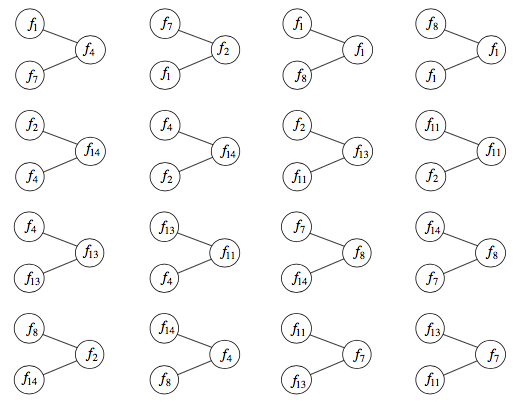
\includegraphics[width=\textwidth]{images/16solutions}

\tiny{Rojas, Ch. 6, Fig. 6.3}
}


\frame{\frametitle{Planes through space}

  \begin{center}
  \begin{tikzpicture}
    [neuron/.style={circle,draw=black,fill=white,inner sep=0pt,minimum size=10mm,outer sep=0.5pt},
    >=stealth',
    scale=0.7,transform shape]
    
    \node          (i01)                              {$x_1$};
    \node          (b00)      [above=10mm of i01]     {$1$};
    
    \node [neuron] (n01)      [right=20mm of i01]     {$\geq 0$};
%    \node [neuron] (b10)      [above=10mm of n01]     {$1$};
%    \node          (inv)      [below=5mm of  n01]     {\ };
%    \node [neuron] (n02)      [below=10mm of n01]     {$f_4$};

    \node          (i02)      [left=20mm of n02]      {$x_2$};
    

%    \node [neuron] (n03)      [right=20mm of n01]     {$f_3$};
%    \node          (inv)      [below=5mm of  n03]     {\ };
%    \node [neuron] (n04)      [right=20mm of n02]     {$f_4$};

%    \node [neuron] (n03)      [right=20mm of inv]     {$f_{14}$};
    
    \node (out)      [right=20mm of n01] {$o$};
    
    \draw [->] (b00) -- (n01) node[sloped, midway, above] {$w_3$} ;
    \draw [->] (i01) -- (n01) node[midway, above] {$w_1$} ;
    \draw [->] (i02) -- (n01) node[sloped, midway, above] {$w_2$} ;
    
%    \draw [->] (b00) -- (n02);
%    \draw [->] (i01) -- (n02);
%    \draw [->] (i02) -- (n02);
%    
%    \draw [->] (n01) -- (n03);
%    \draw [->] (n02) -- (n03);
%    
%    \draw [->] (n01) -- (n04);
%    \draw [->] (n02) -- (n04);
%    
%    \draw [->] (n01) -- (n03);
%    \draw [->] (n02) -- (n03);
    
    \draw [->] (n01) -- (out);
    
  \end{tikzpicture}

\begin{itemize}
\item<+-> $c_1 = x_1 \cdot w_1$
\item<+-> $c_2 = x_2 \cdot w_3$
\item<+-> $c_3 = 1 \cdot w_3$
\item<+->	$\vec{c} = [c_1, c_2, c_3]$ defines a point in 3-dimensional space
\item<+-> $|\vec{c}| = \sqrt{c_1^2 + c_2^2 + c_3^2}$
\item<+-> $\hat{c} = \left[ \frac{c_1}{|\vec{c}|} , \frac{c_2}{|\vec{c}|} , \frac{c_3}{|\vec{c}|} \right]$
\item<+-> $|\hat{c}| = 1$
\end{itemize}
  \end{center}


	
}

\frame{\frametitle{Planes through space}
\begin{tikzpicture}
    \fill[blue!50!gray, opacity=0.7] (0,0) -- (5,0) -- (4,2) -- (1,2) -- cycle;
    \shade[ball color=red] (2.5,0) circle (1);
    \fill[blue!50!gray, opacity=0.7] (0,0) -- (1.5,0) arc (180:360:1 and 0.5) -- (5,0) -- (6,-2) -- (-1,-2) -- cycle;
\end{tikzpicture}
}


\begin{frame}

\note{
This presentation was created and narrated by Lane Schwartz. \\ \ \\
You are free to reproduce and adapt this work under the terms of the Creative Commons Attribution-ShareAlike 4.0 International License.
}

\begin{center}

\includegraphics[scale=0.3]{images/CreativeCommons} \ \ \ \ \ 

\includegraphics[scale=0.3]{images/CreativeCommonsAttribution} \ \ \ \ \ 

\includegraphics[scale=0.3]{images/CreativeCommonsSharealike}
\end{center}

\ \\

%\setbeamertemplate{itemize items}[$+$]
\begin{itemize}
\item[\textbullet] This presentation was created and narrated by Lane Schwartz. \\ \ \\
\item[\textbullet] You are free to reproduce and adapt this work under the terms of the Creative Commons Attribution-ShareAlike 4.0 International License.
\end{itemize}

\end{frame}


%\begin{frame}
\frametitle{Linear unit}

\begin{equation*}
y = b + \sum_i x_i w_i
\end{equation*}


\begin{tikzpicture}
\begin{axis}[ylabel=output,xlabel=weighted input,scale=0.3,grid=major,ytick={0},xtick={0},xmin=-5,xmax=5,ymin=-5,ymax=5]
  \addplot[blue, ultra thick][domain=-10:10] (x,x);
\end{axis}
\end{tikzpicture}

\end{frame}


%\frame {

\begin{center}
$f(x_1,x_2) = \sin(x_1) + x_1*x_2$ \ \ \ \ \ \ \ \ \ \ 
$\bar{x_i} = \frac{\partial f_j}{\partial x_i}$
\pause

\begin{tikzpicture}[>=latex, scale=0.75, transform shape]
\tikzstyle{every node}=[font=\large]
\tikzstyle{every path}=[line width=1pt]

\node[state,rectangle] (fxx) {$f(x_1,x_2)$};
\node[state] (plus) [below=1.5cm of fxx] {$f_5$};
\node[state] (sin) [below left=1.5cm and 0.5cm of plus] {$f_4$};
\node[state] (mul) [below right=1.5cm and 0.5cm of plus] {$f_3$};
\node[state] (x1) [below left=1.5cm and 0.5 cm of sin] {$f_1$};
\node[state] (x2) [below right=1.5cm and 0.5 cm of mul] {$f_2$};

\onslide<+>{
\path[-]
(plus) edge node {} (fxx)
(sin) edge node {} (plus)
(mul) edge node {} (plus)
(x1) edge node {} (sin)
(x1) edge node {} (mul)
(x2) edge node {} (mul);
}

\onslide<+>{
\path[->,blue]
(plus) edge node {} (fxx)
(sin) edge node {} (plus)
(mul) edge node {} (plus)
(x1) edge node {} (sin)
(x1) edge node {} (mul)
(x2) edge node {} (mul);
}

\onslide<.->{
\node[state, draw=none,fill=none,blue] (w1) [left=0.1cm of x1] {$y_1 = f_1(x_1) = x_1$};
\node[state, draw=none,fill=none,blue] (w2) [right=0.1cm of x2] {$y_2 = f_2(x_2) = x_2$};
\node[state, draw=none,fill=none,blue] (w3) [right=0.1cm of mul] {$y_3 = f_3(y_1, y_2) = y_1 \cdot y_2$};
\node[state, draw=none,fill=none,blue] (w4) [left=0.1cm of sin] {$y_4 = f_4(y_1) = \sin(y_1)$};
\node[state, draw=none,fill=none,blue] (w5) [left=0.1cm of plus] {$y_5 = f_5(y_3, y_4) = y_3 + y_4$};
\node[state, draw=none,fill=none,blue] (w6) [right=0.1cm of fxx] {$y_6 = f_6(y_5) = y_5$};
}

\onslide<+>{
\path[<-,red]
(plus) edge node [right] {$\bar{f_6} = \bar{y}_5 = \frac{\partial f_6}{\partial y_5} = 1$} (fxx)
(sin) edge node [left, pos=.6] {$\bar{y}_4 = \frac{\partial f_6}{\partial y_4} = \frac{\partial f_6}{\partial y_5} \frac{\partial y_5}{\partial y_4} = \bar{y}_5 \frac{\partial f_5}{\partial y_4} = \bar{y}_5 \cdot 1 = \bar{y}_5$} (plus)
(mul) edge node [right, pos=.6] {$\bar{y}_3 = \frac{\partial f_6}{\partial y_3} = \frac{\partial f_6}{\partial y_5} \frac{\partial y_5}{\partial y_3} = \bar{y}_5 \frac{\partial f_5}{\partial y_3} = \bar{y}_5 \cdot 1 = \bar{y}_5$} (plus)
(x1) edge node [left,pos=.6] { $\frac{\partial f_6}{\partial y_1} = \bar{y}_4 \frac{\partial y_4}{\partial y_1} = \bar{y}_4\cdot\cos(y_1)$ } (sin)
(x1) edge node [right, pos=.3] {$\bar{y}_{1^b}= \bar{y}_3\cdot y_2$} (mul)
(x2) edge node [right, pos=.6] {$\bar{y}_2 = \bar{y}_3 \frac{\partial y_3}{\partial y_2} = \bar{y}_3\cdot y_1$} (mul);

}

\end{tikzpicture}
\end{center}
}




\frame {

\begin{center}
$f(x_1,x_2) = \sin(x_1) + x_1*x_2$

\ \\

\pause

\begin{tikzpicture}[>=latex, scale=0.75, transform shape]
\tikzstyle{every node}=[font=\large]
\tikzstyle{every path}=[line width=1pt]

\node[state,rectangle] (fxx) {$f(x_1,x_2)$};
\node[state] (plus) [below=1.5cm of fxx] {$+$};
\node[state] (sin) [below left=1.5cm and 0.5cm of plus] {$\sin$};
\node[state] (mul) [below right=1.5cm and 0.5cm of plus] {$*$};
\node[state,rectangle] (x1) [below left=1.5cm and 0.5 cm of sin] {$x_1$};
\node[state,rectangle] (x2) [below right=1.5cm and 0.5 cm of mul] {$x_2$};

\onslide<+>{
\path[-]
(plus) edge node {} (fxx)
(sin) edge node {} (plus)
(mul) edge node {} (plus)
(x1) edge node {} (sin)
(x1) edge node {} (mul)
(x2) edge node {} (mul);
}

\onslide<+>{
\path[->,blue]
(plus) edge node {} (fxx)
(sin) edge node {} (plus)
(mul) edge node {} (plus)
(x1) edge node {} (sin)
(x1) edge node {} (mul)
(x2) edge node {} (mul);
}

\onslide<.->{
\node[state, draw=none,fill=none,blue] (w1) [left=0.1cm of x1] {$y_1 = x_1$};
\node[state, draw=none,fill=none,blue] (w2) [right=0.1cm of x2] {$y_2 = x_2$};
\node[state, draw=none,fill=none,blue] (w3) [right=0.1cm of mul] {$y_3 = y_1 \cdot y_2$};
\node[state, draw=none,fill=none,blue] (w4) [left=0.1cm of sin] {$y_4 = \sin(y_1)$};
\node[state, draw=none,fill=none,blue] (w4) [left=0.1cm of plus] {$y_5 = y_3 + y_4$};
}

\onslide<+>{
\path[<-,red]
(plus) edge node [right] {$\bar{f} = \bar{y}_5 = \frac{\partial f}{\partial y_5} = 1$} (fxx)
(sin) edge node [left, pos=.6] {$\bar{y}_4 = \bar{y}_5 \frac{\partial y_5}{\partial y_4}$} (plus)
(mul) edge node [right, pos=.6] {$\bar{y}_3 = \bar{y}_5 \frac{\partial y_5}{\partial y_3}$} (plus)
(x1) edge node [left,pos=.6] { $\bar{y}_1^a = \bar{y}_4 \frac{\partial y_4}{\partial y_1} = \bar{y}_4\cdot\cos(y_1)$ } (sin)
(x1) edge node [right, pos=.3] {$\bar{y}_1^b= \bar{y}_3\cdot y_2$} (mul)
(x2) edge node [right, pos=.6] {$\bar{y}_2 = \bar{y}_3 \frac{\partial y_3}{\partial y_2} = \bar{y}_3\cdot y_1$} (mul);

}


\end{tikzpicture}
\end{center}
}



\end{document}
